% Generado por a_pdf.py desde reporte.md -- no editar a mano
\documentclass[11pt,a4paper]{article}
\usepackage[utf8]{inputenc}
\usepackage[T1]{fontenc}
\usepackage[spanish,mexico]{babel}
\usepackage{graphicx}
\usepackage[margin=2.5cm]{geometry}
\usepackage{amsmath}
\usepackage{booktabs}
\usepackage{tabularx}
\usepackage{array}
\usepackage{fvextra}
\usepackage{float}
\usepackage{setspace}
\usepackage{parskip}
\usepackage{fancyhdr}
\usepackage{textcomp}
\usepackage[hidelinks]{hyperref}

\onehalfspacing
\setlength{\parskip}{6pt}
\sloppy
\setlength{\emergencystretch}{3em}
\setlength{\headheight}{40pt}
\pagestyle{fancy}
\fancyhf{}
\fancyhead[L]{\includegraphics[width=1cm]{/home/yovick/repos/UAZ-IEI/Assets/UIE.png}}
\fancyhead[R]{\small Comunicaciones Inalámbricas}
\fancyfoot[C]{\thepage}
\renewcommand{\headrulewidth}{0.4pt}

\begin{document}

% ---------------------------- PORTADA -----------------------
\begin{titlepage}
  \thispagestyle{empty}
  \begin{center}
    \vspace*{1cm}
    \includegraphics[width=4.5cm]{/home/yovick/repos/UAZ-IEI/Assets/uaz.png}
    \vspace{0.8cm}

    {\large Universidad Autónoma de Zacatecas}\\[4pt]
    {\large Unidad Académica de Ingeniería Eléctrica}\\[4pt]
    {\normalsize Ingeniería Electrónica Industrial con especialidad en Telecomunicaciones}

    \vspace{1.8cm}
    {\LARGE\bfseries Práctica 3}\\[10pt]
    {\Large\bfseries Caracterización experimental del shadowing log-normal}
  \end{center}

  \vspace{2.2cm}
  \begin{center}
    \begin{tabular}{rl}
      \textbf{Materia:} & Comunicaciones Inalámbricas\\
      \textbf{Docente:} & Dr. Víktor Iván Rodríguez Abdalá\\
      \textbf{Alumno:}  & Arnold Yovick Ríos Zaldívar\\
      \textbf{Fecha:}   & Octubre de 2026\\
    \end{tabular}
  \end{center}
  \vfill
\end{titlepage}

\textbf{Equipo:} RTL-SDR (\texttt{RTL2832U} + tuner \texttt{R820T}), antena telescópica

\textbf{Fuente:} emisora FM 91.5 MHz (no se dispone de transmisor local en 433.9 MHz)

\textbf{Script:} \texttt{practica3.py} (Python; en este repo el análisis se hace en Python en lugar de MATLAB)

\section{Objetivo}

Caracterizar las variaciones lentas de potencia (shadowing o desvanecimiento de gran escala) de un canal inalámbrico real: medir la potencia recibida $P_r(k)$ en 17 posiciones independientes usando una emisora FM como fuente, estimar la media $\mu$ y la desviación estándar $\sigma$ del shadowing local, verificar si las mediciones siguen una distribución aproximadamente normal y obtener su ajuste gaussiano, complementando el modelo de pérdidas por trayectoria.

\section{Fundamento teórico}

Además de la pérdida media por trayectoria, la señal experimenta fluctuaciones lentas por obstáculos (edificios, paredes, mobiliario, vegetación, personas), modeladas por el shadowing log-normal:

\[
PL(d) = PL(d_0) + 10\,n\,\log_{10}\!\left(\frac{d}{d_0}\right) + X_\sigma, \qquad X_\sigma \sim \mathcal{N}(0, \sigma^2)
\]

donde $PL(d_0)$ es la pérdida a la distancia de referencia, $n$ el exponente de pérdidas y $X_\sigma$ una variable aleatoria gaussiana en dB de media cero y desviación estándar $\sigma$.

La potencia recibida de cada medición se estima de las muestras IQ como

\[
P = \frac{1}{M}\sum_{m=1}^{M} |x[m]|^2, \qquad P_r(k) = 10\log_{10}(P)\ \text{(dB)}
\]

y los estimadores muestrales de la media y la desviación estándar son

\[
\mu = \frac{1}{N}\sum_{k=1}^{N} P_r(k), \qquad \sigma = \sqrt{\frac{1}{N-1}\sum_{k=1}^{N}\left(P_r(k)-\mu\right)^2}
\]

El ajuste gaussiano se obtiene por máxima verosimilitud con \texttt{scipy.stats.norm.fit} ($\mu_{fit}$, $\sigma_{fit}$). Si se remueve la pérdida media por trayectoria, las fluctuaciones residuales deben aproximarse a $\mathcal{N}(0,\sigma^2)$, de modo que la normalidad de $P_r$ se contrasta con la prueba de Shapiro-Wilk. Valores típicos de $\sigma$:

\begin{tabularx}{\linewidth}{@{}*{2}{>{\raggedright\arraybackslash}X}@{}}
\toprule
Entorno & $\sigma$ (dB) \\
\midrule
Espacio libre & 2 -- 4 \\
Exterior urbano & 6 -- 10 \\
Interior oficinas & 4 -- 12 \\
Entornos industriales & 8 -- 15 \\
\bottomrule
\end{tabularx}

\section{Desarrollo experimental}

\subsection{Configuración del receptor}

\begin{tabularx}{\linewidth}{@{}*{2}{>{\raggedright\arraybackslash}X}@{}}
\toprule
Parámetro & Valor \\
\midrule
Frecuencia central & 91.5 MHz (emisora FM; no hay transmisor local en 433.9 MHz) \\
Sample rate & 2.4 MSPS \\
Muestras por medición & un bloque IQ de la fuente en vivo \\
Mediciones independientes & 17 \\
Distancia transmisor--receptor & no controlada (fuente lejana) \\
Ganancia (\texttt{--gain}) & auto (la mayor que no recorta el ADC) \\
Ritmo entre mediciones & manual: \texttt{ESPACIO} en cada posición \\
Antena & telescópica del RTL-SDR \\
\bottomrule
\end{tabularx}

\subsection{Escenario}

La fuente es la emisora FM de 91.5 MHz, que llega desde un transmisor lejano; la distancia no se controla. La antena/receptor se reubicó entre mediciones en posiciones cercanas dentro del mismo entorno (pasillo, interior, cerca de paredes y puertas, con presencia/ausencia de personas) para excitar el shadowing local y el multitrayecto, manteniendo la fuente fija.

\subsection{Procedimiento}

\begin{enumerate}
  \item \texttt{python3 practica3.py} abre una sola ventana en vivo con el espectro, la serie de potencias y el histograma con el ajuste gaussiano.
  \item En cada una de las 17 posiciones se pulsa \texttt{ESPACIO} para registrar $P_r(k) = 10\log_{10}(\text{mean}(|x|^2))$ del último bloque IQ; \texttt{r} reinicia las mediciones.
  \item La tecla \texttt{s} guarda las mediciones en \texttt{datos/mediciones.csv} (índice y potencia en dB).
  \item Al guardar se calculan $\mu$, $\sigma$, el ajuste gaussiano, el intervalo de confianza aproximado de $\sigma$ y la prueba de normalidad; todo se guarda en \texttt{datos/resultados.json}.
  \item La misma tecla \texttt{s} genera \texttt{figs/variacion.png} y \texttt{figs/histograma.png}.
\end{enumerate}

\section{Código}

El script completo está en \texttt{practica3.py}. Fragmentos esenciales:

\begin{Verbatim}[breaklines=true,breakanywhere=true,fontsize=\small]
def tecla(self, ev):                                        # al pulsar ESPACIO
    self.registrar(comun.potencia_dbfs(self.app.fuente.ultimo))  # Pr(k)=10*log10(P)
mu, sigma = float(np.mean(Pr)), float(np.std(Pr, ddof=1))                      # mu=mean(Pr); sigma=std(Pr)
mu_fit, sigma_fit = stats.norm.fit(Pr)                                         # pd=fitdist(Pr,'Normal')
p = stats.shapiro(Pr).pvalue                                                   # prueba de normalidad
ax.hist(Pr, bins=10, density=True)                                             # histogram(Pr,'Normalization','pdf')
ax.plot(x, stats.norm.pdf(x, mu_fit, sigma_fit))                               # plot(x, pdf(pd,x))
\end{Verbatim}

\section{Resultados}

La corrida real se realizó con el RTL-SDR y la antena telescópica sintonizados en la emisora FM de \textbf{91.5 MHz}. Se registraron \textbf{17 posiciones} distintas dentro del mismo entorno; la fuente es lejana, así que la distancia no se controló y lo que se caracteriza es el shadowing local (no la pérdida media por trayectoria).

\subsection{Tabla de resultados}

\begin{tabularx}{\linewidth}{@{}*{2}{>{\raggedright\arraybackslash}X}@{}}
\toprule
Parámetro & Valor \\
\midrule
Media $\mu$ (dBFS) & $-$50.29 \\
Desviación $\sigma$ (dB) & 6.29 \\
$\sigma$ del ajuste gaussiano (MLE) & 6.10 \\
N mediciones & 17 \\
Fuente & FM 91.5 MHz \\
Distancia & no controlada (fuente lejana) \\
p-valor (Shapiro-Wilk) & 0.6580 \\
IC 95 \% aproximado de $\sigma$ & [4.11, 8.47] dB \\
Entorno (clasificado por $\sigma$) & exterior urbano / interior con obstáculos \\
\bottomrule
\end{tabularx}

\subsection{Variación de potencia recibida}

\begin{center}
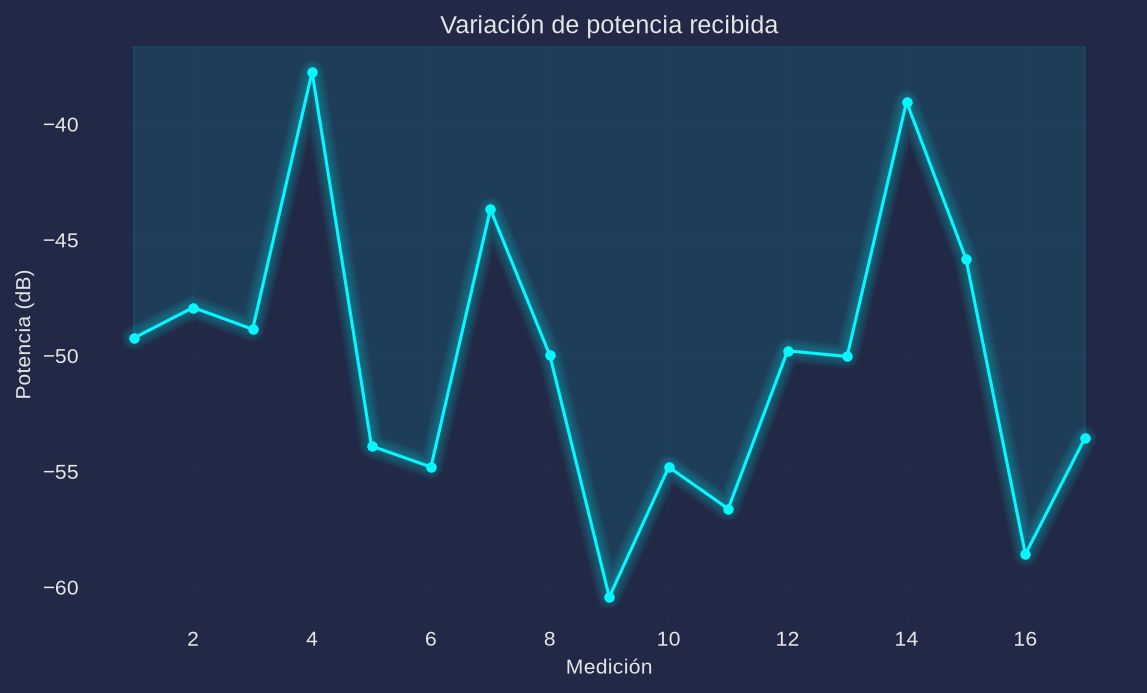
\includegraphics[width=0.9\linewidth]{figs/variacion.png}\\[2pt]
{\small Variación de potencia}
\end{center}

La potencia fluctúa alrededor de $-$50.3 dBFS con excursiones entre aproximadamente $-$60.4 y $-$37.8 dBFS. Esa dispersión de más de 20 dB es la firma del shadowing local y del multitrayecto al mover la antena entre posiciones. No se observa una tendencia monótona porque la distancia a la emisora no cambia de forma controlada; lo que varía es el entorno local.

\subsection{Histograma y ajuste gaussiano}

\begin{center}
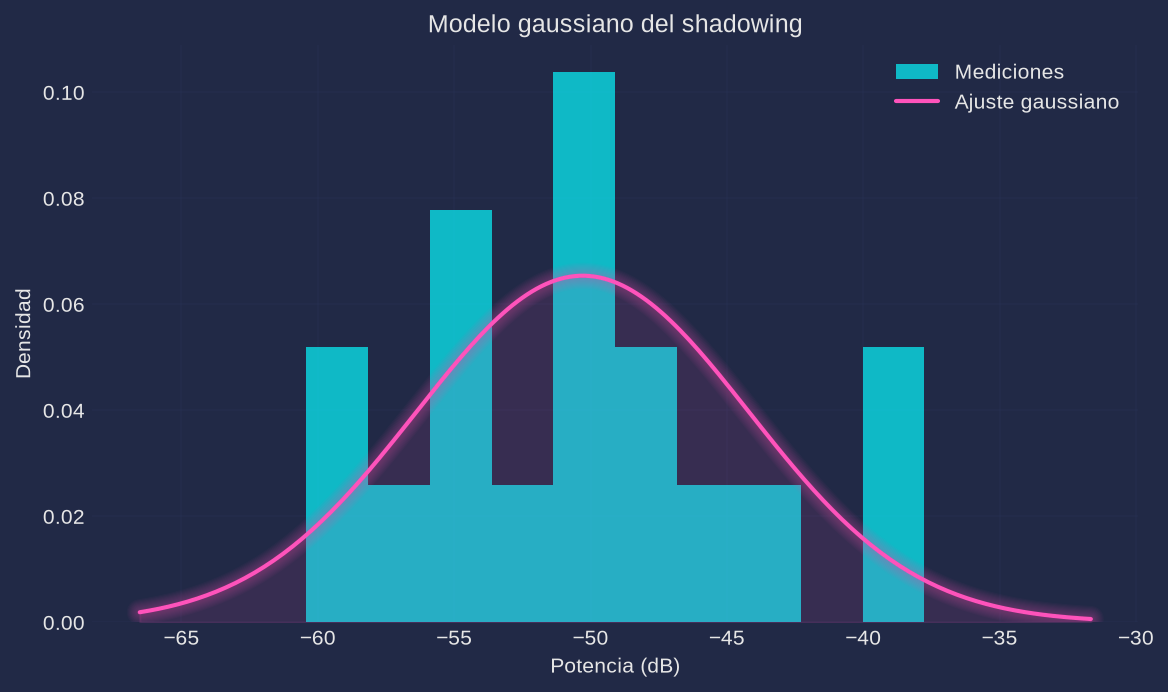
\includegraphics[width=0.9\linewidth]{figs/histograma.png}\\[2pt]
{\small Histograma y ajuste gaussiano}
\end{center}

El histograma normalizado presenta una forma aproximadamente acampanada y la gaussiana ajustada lo sigue de cerca. Con solo 17 muestras el histograma es grueso, pero no se aprecian bimodalidades ni colas pesadas evidentes.

\section{Análisis de resultados}

\begin{itemize}
  \item \textbf{Normalidad:} el p-valor de Shapiro-Wilk (0.6580) es muy superior a 0.05, por lo que \textbf{no se rechaza} la hipótesis de normalidad de $P_r$; las 17 mediciones son compatibles con el modelo log-normal del shadowing. La media del ajuste coincide con la muestral ($-$50.29 dBFS) y la diferencia entre $\sigma$ muestral (6.29 dB) y $\sigma_{fit}$ (6.10 dB) se debe al estimador ($N-1$ vs. máxima verosimilitud).
  \item \textbf{Comparación con la literatura:} $\sigma = 6.29$ dB cae dentro del rango de \textbf{interior de oficinas (4--12 dB)} y en el borde inferior de exterior urbano (6--10 dB). Está por encima del espacio libre (2--4 dB), lo que es consistente con un entorno con paredes, muebles, puertas y personas. El intervalo de confianza [4.11, 8.47] dB es amplio por el tamaño de muestra, pero cubre los valores típicos de interiores.
  \item \textbf{Elementos del entorno:} paredes, puertas y la presencia de personas son los obstáculos que más modifican la potencia recibida; al mover la antena cambian las atenuaciones y las fases de las réplicas multitrayecto, aunque la distancia a la emisora sea prácticamente constante.
  \item \textbf{Pérdida por trayectoria vs. shadowing:} con una emisora lejana no se puede medir el exponente $n$ de path loss, porque la distancia no se controla. Esta práctica caracteriza únicamente la componente aleatoria $X_\sigma$ alrededor de la potencia media local; para el modelo completo $PL(d)$ haría falta un transmisor local a distancias conocidas.
  \item \textbf{Hardware:} la corrida fue real, con el RTL-SDR y la antena; no se usó \texttt{--sim}. Las potencias son dBFS relativas al ADC del receptor, no dBm absolutos, pero $\sigma$ es independiente de la escala y por eso es la métrica robusta del shadowing.
\end{itemize}

\section{Cuestionario}

\begin{enumerate}
  \item \textbf{¿Qué es el shadowing?} Es el desvanecimiento de gran escala: las variaciones lentas de la potencia media recibida causadas por obstáculos que bloquean, absorben o difractan la señal (edificios, paredes, árboles, personas). Se modela superponiendo a la pérdida por trayectoria una variable aleatoria gaussiana en dB, $X_\sigma \sim \mathcal{N}(0,\sigma^2)$, de modo que la potencia lineal resulta log-normal.
\end{enumerate}

\begin{enumerate}
  \item \textbf{¿Qué diferencia existe entre fading de gran escala y de pequeña escala?} El fading de gran escala (shadowing) se debe a obstáculos entre transmisor y receptor y varía lentamente, sobre distancias de muchos metros o cientos de longitudes de onda; afecta la potencia media local. El de pequeña escala (multitrayectoria, Rayleigh/Rician) se debe a la interferencia de réplicas que llegan con retrasos y fases distintas, varía rápidamente (distancias del orden de $\lambda$ o fracciones) y produce desvanecimientos profundos y selectivos en frecuencia.
\end{enumerate}

\begin{enumerate}
  \item \textbf{¿Por qué el shadowing suele modelarse log-normal?} Porque la pérdida en dB producida por cada obstáculo es aditiva: la atenuación total es la suma de muchas contribuciones independientes. Por el teorema central del límite, esa suma tiende a una distribución gaussiana, por lo que la pérdida en dB (el logaritmo de la potencia lineal) es normal; en consecuencia, la potencia lineal sigue una distribución log-normal.
\end{enumerate}

\begin{enumerate}
  \item \textbf{¿Qué representa físicamente $\sigma$?} La dispersión o intensidad del shadowing: cuánto se apartan las mediciones de la pérdida media por trayectoria a una misma distancia. Físicamente resume la agresividad y variabilidad de los obstáculos del entorno: a mayor $\sigma$, mayor incertidumbre en el nivel de potencia recibida y peor predictibilidad del enlace.
\end{enumerate}

\begin{enumerate}
  \item \textbf{¿Cómo afecta el entorno interior al valor de $\sigma$?} Lo incrementa respecto del espacio libre (4--12 dB frente a 2--4 dB), porque en interiores hay gran cantidad y variedad de obstáculos (muros, divisiones, muebles, puertas, personas en movimiento) con atenuaciones muy distintas entre posiciones. Ambientes interiores abiertos o con línea de vista directa tienden al extremo inferior del rango, mientras que oficinas densamente amuebladas o con tráfico de personas se acercan al extremo superior.
\end{enumerate}

\section{Conclusiones}

Se ejecutó la corrida real del análisis de shadowing con el RTL-SDR y la antena telescópica, usando la emisora FM de 91.5 MHz como fuente y 17 posiciones distintas. Se obtuvo $\mu = -50.29$ dBFS, $\sigma = 6.29$ dB, $\sigma_{fit} = 6.10$ dB y $p = 0.6580$ en la prueba de Shapiro-Wilk, de modo que no se rechaza la normalidad y el valor de $\sigma$ es consistente con un entorno interior con obstáculos moderados (4--12 dB). La ausencia de un transmisor local en 433.9 MHz impide medir path loss con distancias controladas; por eso la práctica se limitó al shadowing local con una fuente FM lejana. El procedimiento queda reproducible con \texttt{python3 practica3.py -f 91.5e6 -d 0}, la tecla \texttt{ESPACIO} en cada posición y \texttt{s} para guardar.

\end{document}
